% Options for packages loaded elsewhere
\PassOptionsToPackage{unicode}{hyperref}
\PassOptionsToPackage{hyphens}{url}
%
\documentclass[
  ignorenonframetext,
]{beamer}
\usepackage{pgfpages}
\setbeamertemplate{caption}[numbered]
\setbeamertemplate{caption label separator}{: }
\setbeamercolor{caption name}{fg=normal text.fg}
\beamertemplatenavigationsymbolsempty
% Prevent slide breaks in the middle of a paragraph
\widowpenalties 1 10000
\raggedbottom
\setbeamertemplate{part page}{
  \centering
  \begin{beamercolorbox}[sep=16pt,center]{part title}
    \usebeamerfont{part title}\insertpart\par
  \end{beamercolorbox}
}
\setbeamertemplate{section page}{
  \centering
  \begin{beamercolorbox}[sep=12pt,center]{part title}
    \usebeamerfont{section title}\insertsection\par
  \end{beamercolorbox}
}
\setbeamertemplate{subsection page}{
  \centering
  \begin{beamercolorbox}[sep=8pt,center]{part title}
    \usebeamerfont{subsection title}\insertsubsection\par
  \end{beamercolorbox}
}
\AtBeginPart{
  \frame{\partpage}
}
\AtBeginSection{
  \ifbibliography
  \else
    \frame{\sectionpage}
  \fi
}
\AtBeginSubsection{
  \frame{\subsectionpage}
}

\usepackage{amsmath,amssymb}
\usepackage{lmodern}
\usepackage{iftex}
\ifPDFTeX
  \usepackage[T1]{fontenc}
  \usepackage[utf8]{inputenc}
  \usepackage{textcomp} % provide euro and other symbols
\else % if luatex or xetex
  \usepackage{unicode-math}
  \defaultfontfeatures{Scale=MatchLowercase}
  \defaultfontfeatures[\rmfamily]{Ligatures=TeX,Scale=1}
\fi
\usetheme[]{Antibes}
\usecolortheme{dolphin}
% Use upquote if available, for straight quotes in verbatim environments
\IfFileExists{upquote.sty}{\usepackage{upquote}}{}
\IfFileExists{microtype.sty}{% use microtype if available
  \usepackage[]{microtype}
  \UseMicrotypeSet[protrusion]{basicmath} % disable protrusion for tt fonts
}{}
\makeatletter
\@ifundefined{KOMAClassName}{% if non-KOMA class
  \IfFileExists{parskip.sty}{%
    \usepackage{parskip}
  }{% else
    \setlength{\parindent}{0pt}
    \setlength{\parskip}{6pt plus 2pt minus 1pt}}
}{% if KOMA class
  \KOMAoptions{parskip=half}}
\makeatother
\usepackage{xcolor}
\newif\ifbibliography
\setlength{\emergencystretch}{3em} % prevent overfull lines
\setcounter{secnumdepth}{-\maxdimen} % remove section numbering


\providecommand{\tightlist}{%
  \setlength{\itemsep}{0pt}\setlength{\parskip}{0pt}}\usepackage{longtable,booktabs,array}
\usepackage{calc} % for calculating minipage widths
\usepackage{caption}
% Make caption package work with longtable
\makeatletter
\def\fnum@table{\tablename~\thetable}
\makeatother
\usepackage{graphicx}
\makeatletter
\def\maxwidth{\ifdim\Gin@nat@width>\linewidth\linewidth\else\Gin@nat@width\fi}
\def\maxheight{\ifdim\Gin@nat@height>\textheight\textheight\else\Gin@nat@height\fi}
\makeatother
% Scale images if necessary, so that they will not overflow the page
% margins by default, and it is still possible to overwrite the defaults
% using explicit options in \includegraphics[width, height, ...]{}
\setkeys{Gin}{width=\maxwidth,height=\maxheight,keepaspectratio}
% Set default figure placement to htbp
\makeatletter
\def\fps@figure{htbp}
\makeatother

\titlegraphic{\vspace{-1.5cm}\flushright
\includegraphics[width=2cm,height=2cm]{img/MfPH_logo.png}}
\makeatletter
\makeatother
\makeatletter
\makeatother
\makeatletter
\@ifpackageloaded{caption}{}{\usepackage{caption}}
\AtBeginDocument{%
\ifdefined\contentsname
  \renewcommand*\contentsname{Table of contents}
\else
  \newcommand\contentsname{Table of contents}
\fi
\ifdefined\listfigurename
  \renewcommand*\listfigurename{List of Figures}
\else
  \newcommand\listfigurename{List of Figures}
\fi
\ifdefined\listtablename
  \renewcommand*\listtablename{List of Tables}
\else
  \newcommand\listtablename{List of Tables}
\fi
\ifdefined\figurename
  \renewcommand*\figurename{Figure}
\else
  \newcommand\figurename{Figure}
\fi
\ifdefined\tablename
  \renewcommand*\tablename{Table}
\else
  \newcommand\tablename{Table}
\fi
}
\@ifpackageloaded{float}{}{\usepackage{float}}
\floatstyle{ruled}
\@ifundefined{c@chapter}{\newfloat{codelisting}{h}{lop}}{\newfloat{codelisting}{h}{lop}[chapter]}
\floatname{codelisting}{Listing}
\newcommand*\listoflistings{\listof{codelisting}{List of Listings}}
\makeatother
\makeatletter
\@ifpackageloaded{caption}{}{\usepackage{caption}}
\@ifpackageloaded{subcaption}{}{\usepackage{subcaption}}
\makeatother
\makeatletter
\@ifpackageloaded{tcolorbox}{}{\usepackage[many]{tcolorbox}}
\makeatother
\makeatletter
\@ifundefined{shadecolor}{\definecolor{shadecolor}{rgb}{.97, .97, .97}}
\makeatother
\makeatletter
\makeatother
\ifLuaTeX
  \usepackage{selnolig}  % disable illegal ligatures
\fi
\usepackage[style=authoryear]{biblatex}
\addbibresource{refs.bib}
\IfFileExists{bookmark.sty}{\usepackage{bookmark}}{\usepackage{hyperref}}
\IfFileExists{xurl.sty}{\usepackage{xurl}}{} % add URL line breaks if available
\urlstyle{same} % disable monospaced font for URLs
\hypersetup{
  pdftitle={Using statistical methods and reproducible tools to gain new insights from biomedical and public health data},
  hidelinks,
  pdfcreator={LaTeX via pandoc}}

\title{Using statistical methods and reproducible tools to gain new
insights from biomedical and public health data}
\author{Ariel Mundo Ortiz}
\date{3/15/23}
\institute{Centre de Recherches Mathematiques, Université de Montréal
\newline \newline \Large \textbf{MfPH Next Generation Seminar Series}}

\begin{document}
\frame{\titlepage}
\ifdefined\Shaded\renewenvironment{Shaded}{\begin{tcolorbox}[frame hidden, sharp corners, interior hidden, enhanced, borderline west={3pt}{0pt}{shadecolor}, breakable, boxrule=0pt]}{\end{tcolorbox}}\fi

\begin{frame}{Introduction}
\protect\hypertarget{introduction}{}
\begin{itemize}[<+->]
\item
  Data is the core of research. However, data is not information, as it
  needs to be processed before we can get information from it.
\item
  This is specially true in the case of health research: public health,
  or biomedical data can be complex, and decisions along the analysis
  can result in different interpretations.
\item
  In this talk I will focus on two examples that showcase how we can get
  more insight from looking at data from a different perspective.
\end{itemize}
\end{frame}

\hypertarget{the-case-of-public-health-data-covid-19-vaccination}{%
\section{The Case of Public Health Data: COVID-19
Vaccination}\label{the-case-of-public-health-data-covid-19-vaccination}}

\begin{frame}{COVID-19: Why?}
\protect\hypertarget{covid-19-why}{}
\begin{itemize}[<+->]
\item
  The pandemic is still ongoing
\item
  COVID-19 vaccination has been an important component of public health
  strategies aimed at managing the pandemic.
\item
  However, COVID-19 vaccination has not been equal across different
  population segments.
\end{itemize}

\pause

\begin{itemize}[<+->]
\item
  Individuals with lower income, and those belonging to a racial/ethnic
  minority have had lower vaccination uptake
  \footcite{nafilyan2021}\(^{,}\)\footcite{gerretsen2021}.
\item
  This is important because these differences in vaccination uptake have
  implications on virus transmission.
\end{itemize}
\end{frame}

\begin{frame}{COVID-19: The Case of Ontario}
\protect\hypertarget{covid-19-the-case-of-ontario}{}
\begin{itemize}[<+->]
\item
  The Fields Institute collected some very nice data regarding COVID-19
  vaccination in Ontario: the \emph{Survey of COVID-19 related
  Behaviours and Attitudes}.

  \begin{itemize}[<+->]
  \tightlist
  \item
    The survey ran between late 2021 and early 2022 and collected
    socio-demographic information along with self-reported vaccination
    status (``Have you received the first dose of the Covid vaccine?'')
  \end{itemize}
\end{itemize}
\end{frame}

\begin{frame}{COVID-19: The Case of Ontario}
\protect\hypertarget{covid-19-the-case-of-ontario-1}{}
\hypertarget{tbl-covariates}{}
\begin{longtable}[]{@{}
  >{\raggedright\arraybackslash}p{(\columnwidth - 2\tabcolsep) * \real{0.3014}}
  >{\raggedright\arraybackslash}p{(\columnwidth - 2\tabcolsep) * \real{0.6986}}@{}}
\caption{\label{tbl-covariates}Selected socio-economic factors from the
survey}\tabularnewline
\toprule()
\begin{minipage}[b]{\linewidth}\raggedright
Variable
\end{minipage} & \begin{minipage}[b]{\linewidth}\raggedright
Levels
\end{minipage} \\
\midrule()
\endfirsthead
\toprule()
\begin{minipage}[b]{\linewidth}\raggedright
Variable
\end{minipage} & \begin{minipage}[b]{\linewidth}\raggedright
Levels
\end{minipage} \\
\midrule()
\endhead
Age group & 16-34,35-54,55 and over \\
Income bracket (CAD) & under 25,000, 25,000-59,999, 60,000 and above \\
Race/ethnicity & Arab/Middle Eastern, Black, East Asian/Pacific
Islander, Indigenous, Latin American, Mixed, South Asian, White
Caucasian, Other \\
\bottomrule()
\end{longtable}
\end{frame}

\begin{frame}{COVID-19: The Case of Ontario}
\protect\hypertarget{covid-19-the-case-of-ontario-2}{}
\begin{itemize}[<+->]
\item
  Other studies have analyzed the dependency on vaccination status using
  socio-economic data.
\item
  We could do the same, but what else can we get from this data?

  \begin{itemize}[<+->]
  \tightlist
  \item
    There have been some interesting changes in Ontario with regard to
    healthcare.
  \end{itemize}
\end{itemize}
\end{frame}

\begin{frame}{COVID-19: The Case of Ontario}
\protect\hypertarget{covid-19-the-case-of-ontario-3}{}
\begin{itemize}[<+->]
\item
  Between 2006 and 2019, Ontario was geographically divided in ``Local
  Health Integration Networks'' (LHINs).
\item
  LHINs were essentially geographic intra-provincial divisions that
  determined where you could get health care.
\item
  There were 14 LHINs, with additional subdivisions.
\end{itemize}
\end{frame}

\begin{frame}{COVID-19: The Case of Ontario}
\protect\hypertarget{covid-19-the-case-of-ontario-4}{}
\begin{itemize}[<+->]
\item
  Problems with the LHINs:
\item
  In multiple cases, the boundary of a LHIN did not match a municipal
  boundary.

  \begin{itemize}[<+->]
  \item
    One part of a city would be in a LHIN whereas another part of it
    would be in another LHIN.
  \item
    Weakness in this approach due to complexity, lack of funding and
    bureaucracy were identified \footcite{tsasis2012}.
  \end{itemize}
\end{itemize}
\end{frame}

\begin{frame}{COVID-19: The Case of Ontario}
\protect\hypertarget{covid-19-the-case-of-ontario-5}{}
\begin{itemize}[<+->]
\item
  In late 2019, Ontario adopted the Health Regions approach for
  healthcare and phased out the Local Health Integration Network (LHIN)
  approach.
\item
  The change is relatively new. Multiple challenges:

  \begin{itemize}[<+->]
  \tightlist
  \item
    Data for the Health Regions is not available from the Census.
  \item
    \textbf{Have the Health Regions helped in reducing disparities in
    healthcare in the province?}
  \end{itemize}
\end{itemize}
\end{frame}

\begin{frame}{COVID-19: The Case of Ontario}
\protect\hypertarget{covid-19-the-case-of-ontario-6}{}
\begin{columns}[T]
\begin{column}{0.5\textwidth}
\begin{figure}

{\centering 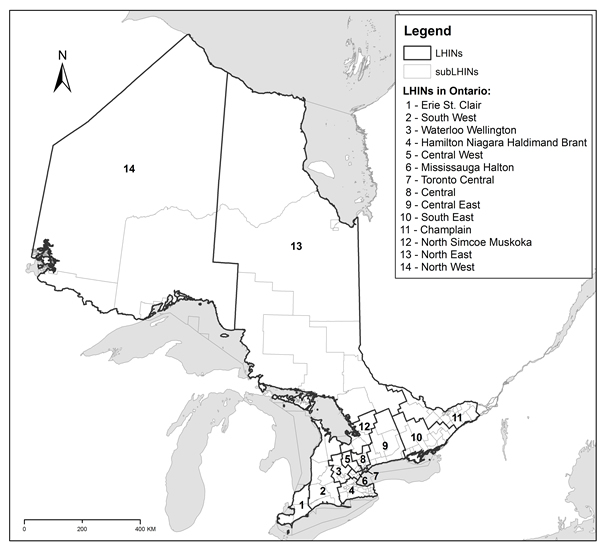
\includegraphics[width=1\textwidth,height=\textheight]{img/LHIN_map.jpg}

}

\caption{Ontario LHINs (Crighton et al.~2015)}

\end{figure}
\end{column}

\begin{column}{0.5\textwidth}
\pause

\begin{figure}

{\centering 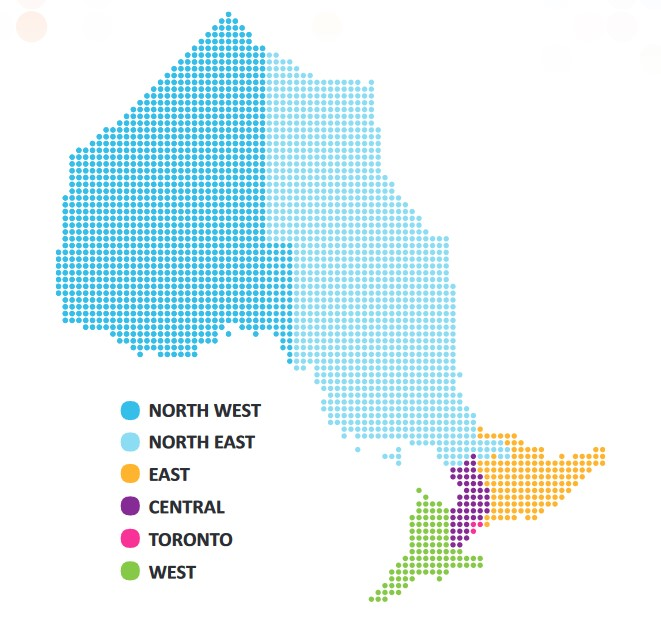
\includegraphics[width=1\textwidth,height=\textheight]{img/ON_HR_map.jpg}

}

\caption{Ontario Health Regions (Ontario Business Health Plan
2022-2023)}

\end{figure}
\end{column}
\end{columns}
\end{frame}

\begin{frame}{COVID-19: The Case of Ontario}
\protect\hypertarget{covid-19-the-case-of-ontario-7}{}
\begin{itemize}[<+->]
\tightlist
\item
  Where in Ontario did responses come from?
\end{itemize}

\begin{figure}

{\centering 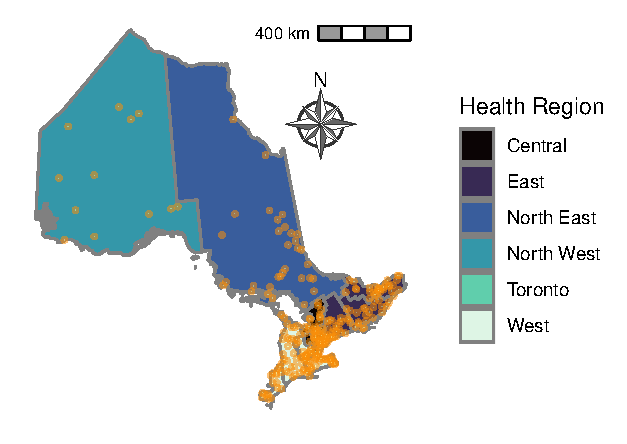
\includegraphics[width=0.7\textwidth,height=0.7\textheight]{img/map.pdf}

}

\caption{\label{fig-map}Geographic representation of the survey data
collected by the Fields Institute}

\end{figure}
\end{frame}

\begin{frame}{COVID-19: The Case of Ontario}
\protect\hypertarget{covid-19-the-case-of-ontario-8}{}
\begin{itemize}[<+->]
\tightlist
\item
  Therefore, we decided to integrate the different Health Regions in our
  analysis to determine the odds of vaccination.
\end{itemize}

\begin{equation}\protect\hypertarget{eq-model1}{}{
\begin{aligned}
\log \left( \frac{p\textrm{(vac)}}{1-p\textrm{(vac)}} \right) = \beta_0+ \beta_{1}\textrm{(Age group)} +\beta_{2} \textrm{ Race} +\\ \beta_3 \textrm{ Health Region} + \beta_4 \textrm{ Income}+ \\ \\ \beta_5\textrm{(Health Region} \times \textrm{Race)} + \beta_6 \textrm{ (Income} \times \textrm{Race)}
\end{aligned}
}\label{eq-model1}\end{equation}
\end{frame}

\begin{frame}{Results}
\protect\hypertarget{results}{}
\tiny
\renewcommand{\arraystretch}{0.5}

\hypertarget{tbl-model}{}
\begin{longtable}{lccc}
\caption{\label{tbl-model}\textbf{Selected} Multivariable Regression Results}\tabularnewline

\toprule
\textbf{Characteristic} & \textbf{OR} & \textbf{95\% CI} & \textbf{p-value}\\
\midrule
\endfirsthead
\multicolumn{4}{@{}l}{\textit{(continued)}}\\
\toprule
\textbf{Characteristic} & \textbf{OR} & \textbf{95\% CI} & \textbf{p-value}\\
\midrule
\endhead

\endfoot
\bottomrule
\endlastfoot
\textbf{Income (CAD)} &  &  & \\
\hspace{1em}60000 and above & — & — & \\
\hspace{1em}25000-59999 & 0.59 & 0.39, 0.89 & 0.011\\
\hspace{1em}under 25000 & 0.37 & 0.25, 0.56 & <0.001\\
\textbf{Race} &  &  & \\
\hspace{1em}White/Caucasian & — & — & \\
\hspace{1em}Arab/Middle Eastern & 0.31 & 0.14, 0.69 & 0.004\\
\hspace{1em}Black & 0.32 & 0.17, 0.60 & <0.001\\
\hspace{1em}East Asian/Pacific Islander & 1.15 & 0.50, 2.66 & 0.7\\
\hspace{1em}Indigenous & 0.44 & 0.19, 1.02 & 0.056\\
\hspace{1em}Latin Aamerican & 0.28 & 0.11, 0.67 & 0.004\\
\hspace{1em}Mixed & 0.64 & 0.25, 1.65 & 0.4\\
\hspace{1em}Other & 0.22 & 0.12, 0.41 & <0.001\\
\hspace{1em}South Asian & 0.91 & 0.49, 1.69 & 0.8\\
\textbf{Health Region} &  &  & \\
\hspace{1em}Toronto & — & — & \\
\hspace{1em}Central & 1.47 & 0.92, 2.35 & 0.11\\
\hspace{1em}East & 1.42 & 0.90, 2.23 & 0.13\\
\hspace{1em}West & 1.55 & 1.05, 2.30 & 0.029\\
\textbf{Income and Race} &  &  & \\
\hspace{1em}25000-59999 * Arab/Middle Eastern & 1.79 & 0.67, 4.83 & 0.2\\
\hspace{1em}under 25000 * Arab/Middle Eastern & 3.05 & 1.26, 7.39 & 0.013\\
\hspace{1em}25000-59999 * Black & 1.34 & 0.59, 3.05 & 0.5\\
\hspace{1em}under 25000 * Black & 3.19 & 1.45, 6.99 & 0.004\\
\hspace{1em}25000-59999 * East Asian/Pacific Islander & 0.42 & 0.17, 1.05 & 0.062\\
\hspace{1em}under 25000 * East Asian/Pacific Islander & 1.16 & 0.47, 2.86 & 0.8\\
\hspace{1em}25000-59999 * Indigenous & 1.36 & 0.48, 3.89 & 0.6\\
\hspace{1em}under 25000 * Indigenous & 1.45 & 0.55, 3.80 & 0.5\\
\hspace{1em}25000-59999 * Latin American & 1.24 & 0.45, 3.43 & 0.7\\
\end{longtable}
\end{frame}

\begin{frame}{Results}
\protect\hypertarget{results-1}{}
\tiny
\renewcommand{\arraystretch}{0.5}

\hypertarget{tbl-model1}{}
\begin{longtable}{lccc}
\toprule
\textbf{Characteristic} & \textbf{OR} & \textbf{95\% CI} & \textbf{p-value}\\
\midrule

\hspace{1em}under 25000 * Latin American & 2.80 & 1.04, 7.51 & 0.041\\
\hspace{1em}25000-59999 * Mixed & 0.85 & 0.32, 2.26 & 0.7\\
\hspace{1em}under 25000 * Mixed & 1.10 & 0.37, 3.27 & 0.9\\
\hspace{1em}25000-59999 * Other & 6.93 & 2.65, 18.1 & <0.001\\
\hspace{1em}under 25000 * Other & 4.59 & 2.33, 9.05 & <0.001\\
\hspace{1em}25000-59999 * South Asian & 1.20 & 0.51, 2.85 & 0.7\\
\hspace{1em}under 25000 * South Asian & 2.00 & 0.93, 4.30 & 0.077\\
\textbf{Race and Health Region} &  &  & \\
\hspace{1em}Arab/Middle Eastern * Central & 0.66 & 0.26, 1.70 & 0.4\\
\hspace{1em}Black * Central & 0.44 & 0.19, 0.98 & 0.046\\
\hspace{1em}East Asian/Pacific Islander * Central & 0.98 & 0.38, 2.53 & >0.9\\
\hspace{1em}Mixed * East & 0.91 & 0.28, 3.03 & 0.9\\
\hspace{1em}other * East & 1.05 & 0.39, 2.83 & >0.9\\
\hspace{1em}South Asian * East & 0.52 & 0.19, 1.45 & 0.2\\
\hspace{1em}Arab/Middle Eastern * West & 1.00 & 0.37, 2.73 & >0.9\\
\hspace{1em}Black * West & 0.76 & 0.32, 1.80 & 0.5\\
\hspace{1em}East Asian/Pacific Islander * West & 0.52 & 0.20, 1.34 & 0.2\\
\hspace{1em}Indigenous * West & 0.39 & 0.14, 1.09 & 0.073\\
\hspace{1em}Latin American * West & 0.94 & 0.32, 2.72 & >0.9\\
\hspace{1em}Mixed * West & 0.37 & 0.12, 1.16 & 0.089\\
\hspace{1em}Other * West & 0.41 & 0.18, 0.93 & 0.032\\
\hspace{1em}South Asian * West & 0.41 & 0.18, 0.95 & 0.037\\*
\multicolumn{4}{l}{\rule{0pt}{1em}\textsuperscript{1} OR = Odds Ratio, CI = Confidence Interval}\\
\end{longtable}
\end{frame}

\begin{frame}{How do we interpret this?}
\protect\hypertarget{how-do-we-interpret-this}{}
\begin{itemize}[<+->]
\item
  Our results show that there were disparities in vaccination uptake in
  Ontario.
\item
  People in certain racial minority groups had lower odds of vaccination
  than White/Caucasian individuals.
\item
  However, individuals that identified with a racial/ethnic minority and
  that were in a low household income bracket (\textless60k CAD) had
  higher odds of vaccination than individuals with a high household
  income.
\item
  This is likely caused by the type of occupation: people in racial
  minorities, and those with a low household income work in essential
  occupations (gas station workers, grocery store workers, agricultural
  workers) \footcite{hawkins2020}, and thus potentially got the vaccine
  to be able to work.
\end{itemize}
\end{frame}

\begin{frame}{How do we interpret this?}
\protect\hypertarget{how-do-we-interpret-this-1}{}
\begin{itemize}[<+->]
\item
  But there are also intra-provincial differences in vaccine uptake
  within the Health Regions:

  \begin{itemize}[<+->]
  \item
    For example, South Asian individuals in the West Health Region had
    lower odds of vaccination that in other Health Regions.
  \item
    These results provide a more comprehensive assessment of COVID-19
    vaccination rates within Ontario, as they showed that certain
    minority groups within specific income brackets and certain Health
    Regions had differences in vaccination.
  \end{itemize}
\end{itemize}
\end{frame}

\begin{frame}{Conclusions}
\protect\hypertarget{conclusions}{}
\begin{itemize}[<+->]
\item
  Data cleaning is \textbf{important}\}

  \begin{itemize}[<+->]
  \tightlist
  \item
    Unifying geographical data can be challenging
  \item
    Specially because most data relies on legacy information from the
    LHINs
  \end{itemize}
\item
  A more granular view of data (in this case, examining differences
  within Health Region, Income and Race) can provide insight for public
  policy development.
\item
  There is a need for future studies that examine more in detail these
  differences and can provide a rationale.
\end{itemize}
\end{frame}

\hypertarget{the-case-of-biomedical-data}{%
\section{The Case of Biomedical
Data}\label{the-case-of-biomedical-data}}

\begin{frame}{Longitudinal Data}
\protect\hypertarget{longitudinal-data}{}
\begin{itemize}[<+->]
\tightlist
\item
  Biomedical studies often collect longitudinal data to see the effect
  of an intervention over time:

  \begin{itemize}[<+->]
  \tightlist
  \item
    How a chemotherapy treatment changes the metabolism of a tumor
  \item
    How the concentration of a drug changes over time in the blood
  \end{itemize}
\item
  \textcolor{red}{How is this data typically analyzed?}
\end{itemize}
\end{frame}

\begin{frame}{Linear Models}
\protect\hypertarget{linear-models}{}
\begin{equation}\protect\hypertarget{eq-model2}{}{
\begin{aligned}
y_{ijt} = \beta_0+\beta_1 \times treatment_{j} +\beta_2 \times time_{t} +\\ \beta_3 \times time_{t}\times treatment_{j}+\varepsilon_{ijt}\\ 
\end{aligned}
}\label{eq-model2}\end{equation}

where,

\(y_{ijt}\): is the response for subject \(i\) in treatment group \(j\)
at time \(t\)

\pause

\(\beta_0\): the mean group value

\pause

\(time_t\), \(treatment_j\): fixed effects

\pause

\(\beta_1, \beta_2\) and \(\beta_3\): linear slopes of the fixed
effects.

\pause

\(\varepsilon_{ijt}\): error, assumed to be \(\sim N(0,\sigma^2)\)

\pause

A LMEM follows the same exact structure, only incorporates a random
effect \(\alpha_{ij}\), which allows for different intercepts.
\end{frame}

\begin{frame}{Trends Over Time}
\protect\hypertarget{trends-over-time}{}
\begin{columns}[T]
\begin{column}{0.5\textwidth}
\begin{figure}

{\centering 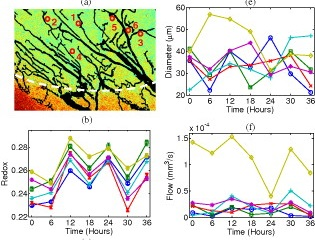
\includegraphics[width=1\textwidth,height=\textheight]{img/Skala.jpg}

}

\caption{Tumor imaging data (Skala et al.~2010)}

\end{figure}
\end{column}

\begin{column}{0.5\textwidth}
\begin{figure}

{\centering 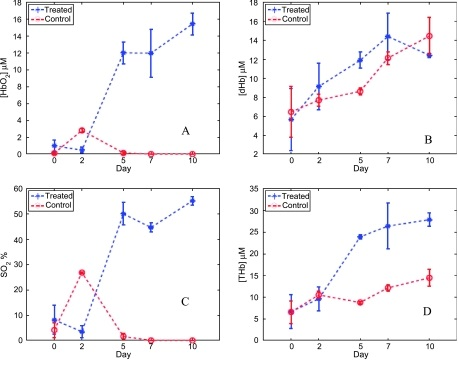
\includegraphics[width=1\textwidth,height=\textheight]{img/Vishwanath.jpg}

}

\caption{Tumor oxygenation data (Vishwanath et al.~2009)}

\end{figure}
\end{column}
\end{columns}
\end{frame}

\begin{frame}{Trends Over Time}
\protect\hypertarget{trends-over-time-1}{}
\begin{itemize}[<+->]
\item
  The issue in those data is that the trends are not linear, and
  therefore, a linear model will miss changes in the signal where some
  metabolic or physiological relevant change is taking place.
\item
  Polynomial effects can be used, but they create biases at the
  boundaries of the covariates\footcite{beck1998}.
\end{itemize}
\end{frame}

\begin{frame}{Generalized Additive Models (GAMs)}
\protect\hypertarget{generalized-additive-models-gams}{}
\begin{equation}\protect\hypertarget{eq-GAM}{}{
y_{ijt}=\beta_0+ \beta_1 \times treatment_j+f(time_t\mid \beta_j)+\varepsilon_{ijt}
}\label{eq-GAM}\end{equation}

\begin{itemize}[<+->]
\tightlist
\item
  The change of \(y_{ijt}\) over time is represented by the \emph{smooth
  function} \(f(time_t\mid \beta_j)\) with inputs as the covariates
  \(time_t\) and parameters \(\beta_j\).
\end{itemize}

\pause

\begin{itemize}[<+->]
\tightlist
\item
  We can use a \emph{basis function} to estimate the smooth function.
\end{itemize}

\pause

\begin{itemize}[<+->]
\tightlist
\item
  Splines are helpful as basis functions: Thin plate regression splines
  (TPRS) are computationally efficient, and the underlying principle is
  that of polynomial pieces ``joined'' together
\end{itemize}
\end{frame}

\begin{frame}{How GAMs work}
\protect\hypertarget{how-gams-work}{}
\begin{figure}

{\centering 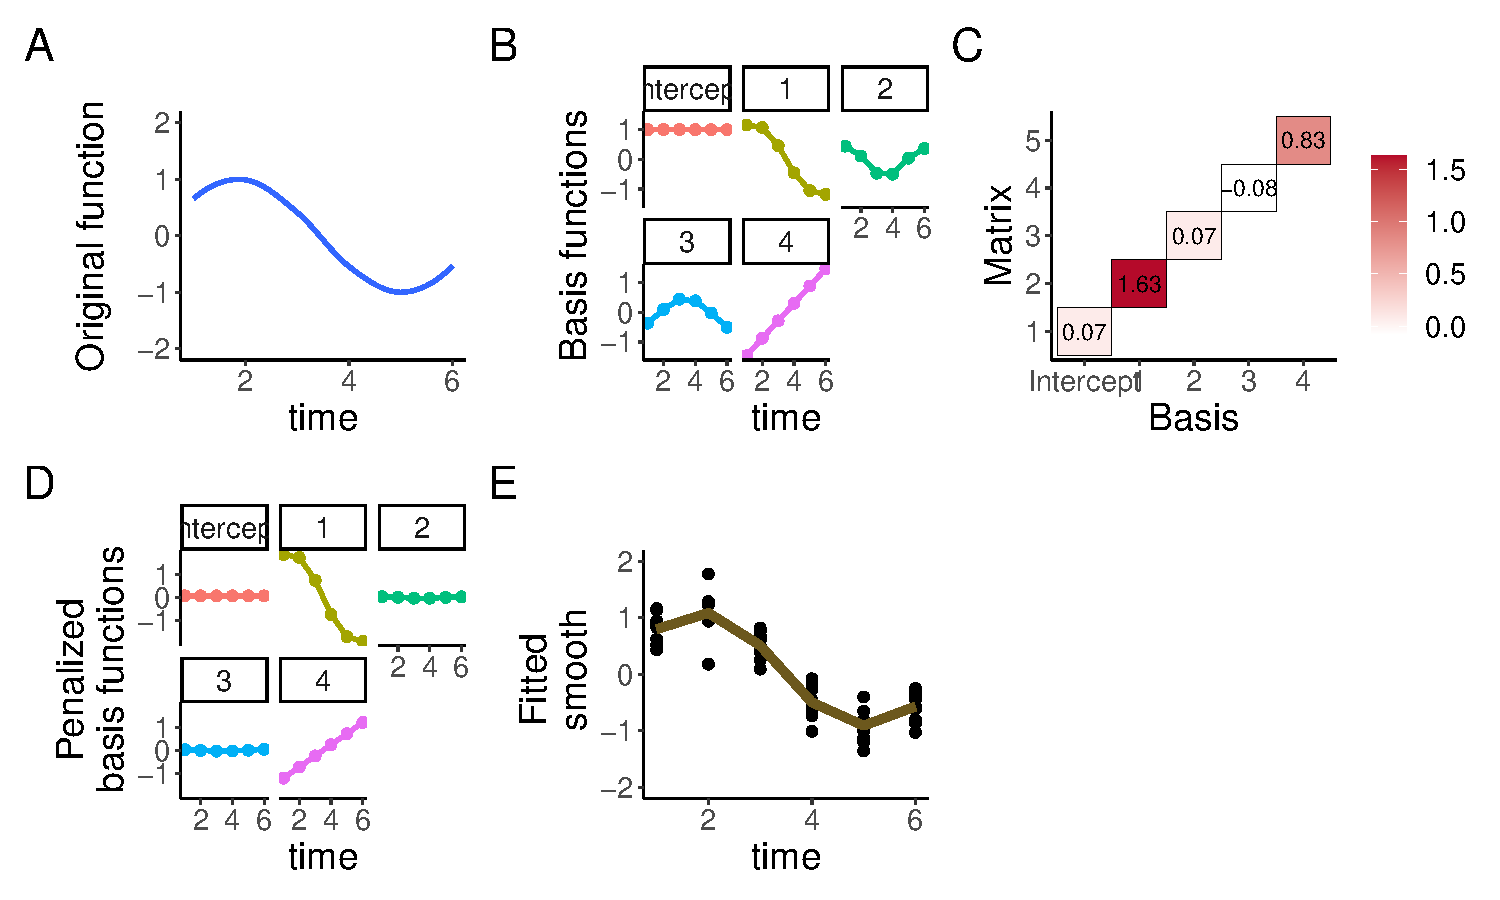
\includegraphics{MfPH_Next_Generation_AM_March_2023_files/figure-beamer/basis-functions-plot-1.pdf}

}

\caption{Fitting process of a GAM.}

\end{figure}
\end{frame}

\begin{frame}{An Example}
\protect\hypertarget{an-example}{}
\begin{itemize}[<+->]
\tightlist
\item
  Simulated data from a study on radiotherapy in a mouse model of
  melanoma \footcite{sen2011}.
\end{itemize}

\begin{figure}

{\centering 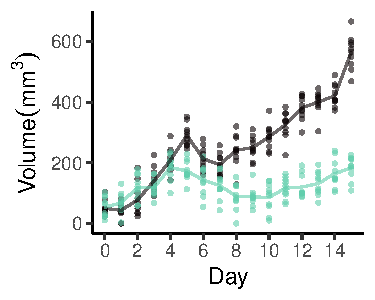
\includegraphics{MfPH_Next_Generation_AM_March_2023_files/figure-beamer/simulated-data-1.pdf}

}

\caption{Tumor volume in two groups of tumors under radiotherapy}

\end{figure}
\end{frame}

\begin{frame}{Fitting a GAM}
\protect\hypertarget{fitting-a-gam}{}
\begin{figure}

{\centering 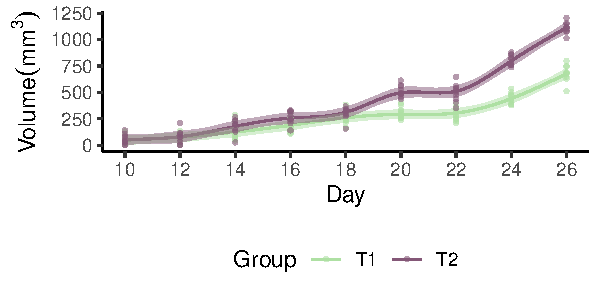
\includegraphics{MfPH_Next_Generation_AM_March_2023_files/figure-beamer/model-1.pdf}

}

\caption{GAM fitted to simulated data}

\end{figure}

\begin{itemize}[<+->]
\item
  The model captures the trend of the data
\item
  We can furthermore compare the trends.
\end{itemize}
\end{frame}

\begin{frame}{Differences}
\protect\hypertarget{differences}{}
\begin{figure}

{\centering 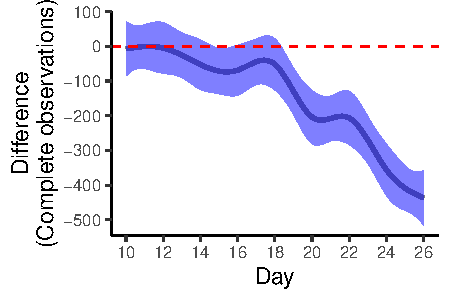
\includegraphics{MfPH_Next_Generation_AM_March_2023_files/figure-beamer/differences-1.pdf}

}

\caption{Pairwise comparisons between smooths}

\end{figure}

\begin{itemize}[<+->]
\item
  We can compare the smooths for each group. Here, we see that T2 is
  significantly higher after \approx day 18.
\item
  This can give an idea of further explorations of biological processes
  that might be driving this difference (e.g., hypoxia, metabolic
  changes, vascular development).
\end{itemize}
\end{frame}

\begin{frame}{Conclusions}
\protect\hypertarget{conclusions-1}{}
\begin{itemize}[<+->]
\item
  GAMs are useful to analyze longitudinal data because they provide:

  \begin{itemize}[<+->]
  \item
    A model that captures non-linear trends in the data
  \item
    This allows to examine specific time points that might be of
    interest, where metabolic, or physiological relevant changes might
    be occuring
  \item
    Lets the data speak for itself
  \end{itemize}
\end{itemize}
\end{frame}

\begin{frame}{Addressing Reproducibility}
\protect\hypertarget{addressing-reproducibility}{}
\begin{itemize}[<+->]
\item
  There is an ongoing need of making papers reproducible.
\item
  This is specially important in the case of data/methods of health
  research.

  \begin{itemize}[<+->]
  \tightlist
  \item
    Otherwise, tools cannot be used by others.
  \end{itemize}
\item
  How are we addressing this in our research?
\end{itemize}
\end{frame}

\begin{frame}{Addressing Reproducibility}
\protect\hypertarget{addressing-reproducibility-1}{}
\begin{itemize}[<+->]
\item
  Using GitHub to share:

  \begin{itemize}[<+->]
  \item
    Data: Making publicly available the datasets used
  \item
    Methods: Sharing the code used for statistical analyses
  \end{itemize}
\item
  In synthesis, sharing all the information used to create a paper such
  that anyone can re-create the analysis, results, and the paper itself
  from the files provided.
\end{itemize}
\end{frame}

\begin{frame}{Addressing Reproducibility}
\protect\hypertarget{addressing-reproducibility-2}{}
\begin{itemize}[<+->]
\item
  For GAMs \url{https://github.com/aimundo/GAMs-biomedical-research}
\item
  COVID-19: Work is ongoing, but repository will be ready when paper is
  submitted
\end{itemize}
\end{frame}

\begin{frame}{Conclusion}
\protect\hypertarget{conclusion}{}
\begin{itemize}[<+->]
\item
  There is an ongoing need of analyzing public health data to address
  important disparities in areas such as vaccination.
\item
  Semi-parametric statistical to analyze biomedical/public health
  longitudinal data, such as GAMs can provide better insight on periods
  where important biological changes might occur.
\end{itemize}
\end{frame}

\begin{frame}{Acknowledgements}
\protect\hypertarget{acknowledgements}{}
\begin{columns}[T]
\begin{column}{0.5\textwidth}
\begin{itemize}
\item
  \textcolor{blue}{The Nasri Lab (Université de Montréal)}

  \begin{itemize}
  \item
    Bouchra Nasri, PhD (PI)
  \item
    Idriss Sekkak, PhD
  \item
    Rado Ramasy
  \item
    Fatima El-Mousawi
  \item
    Rawda Berkat
  \end{itemize}
\end{itemize}

\break

\begin{itemize}
\item
  \textcolor{blue}{The Muldoon Lab (University of Arkansas)}

  \begin{itemize}
  \tightlist
  \item
    Timothy J. Muldoon (PI)
  \end{itemize}
\item
  John R. Tipton (Los Alamos National Laboratory)
\end{itemize}
\end{column}

\begin{column}{0.5\textwidth}

\includegraphics[width=0.8\textwidth,height=\textheight]{img/crm_logo.png}

\includegraphics[width=1\textwidth,height=\textheight]{img/Fields_MfPH.jpg}

\includegraphics[width=0.5\textwidth,height=\textheight]{img/ABI.png}

\includegraphics[width=0.3\textwidth,height=\textheight]{img/nsf.png}
\end{column}
\end{columns}
\end{frame}


\begin{frame}[allowframebreaks]{}
  \bibliographytrue
  \printbibliography[heading=none]
\end{frame}


\end{document}
